\subsection{Diagrama de clases}
Se muestra el diagrama de clases que compone al arbol sintáctico, cada clase se corresponde con un componente del lenguaje.
Se repite la clase Nodo para facilitar la visualización.

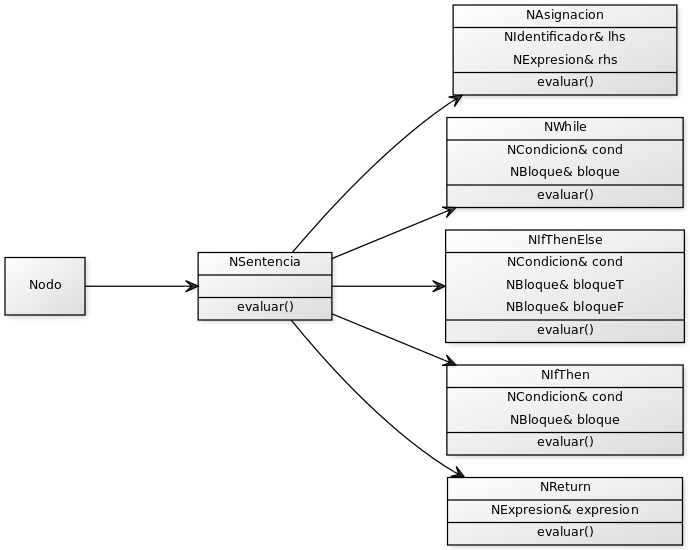
\includegraphics[width=0.9\textwidth,height=0.9\textheight,keepaspectratio]{imgs/clases1.png}

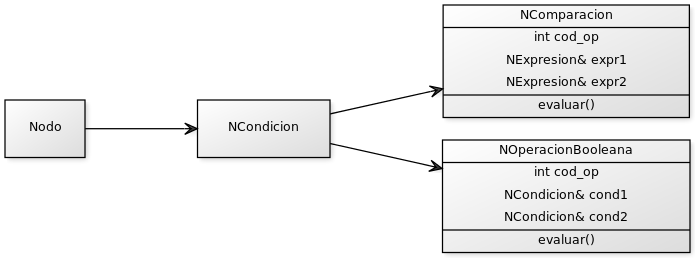
\includegraphics[width=0.9\textwidth,height=0.9\textheight,keepaspectratio]{imgs/clases2.png}

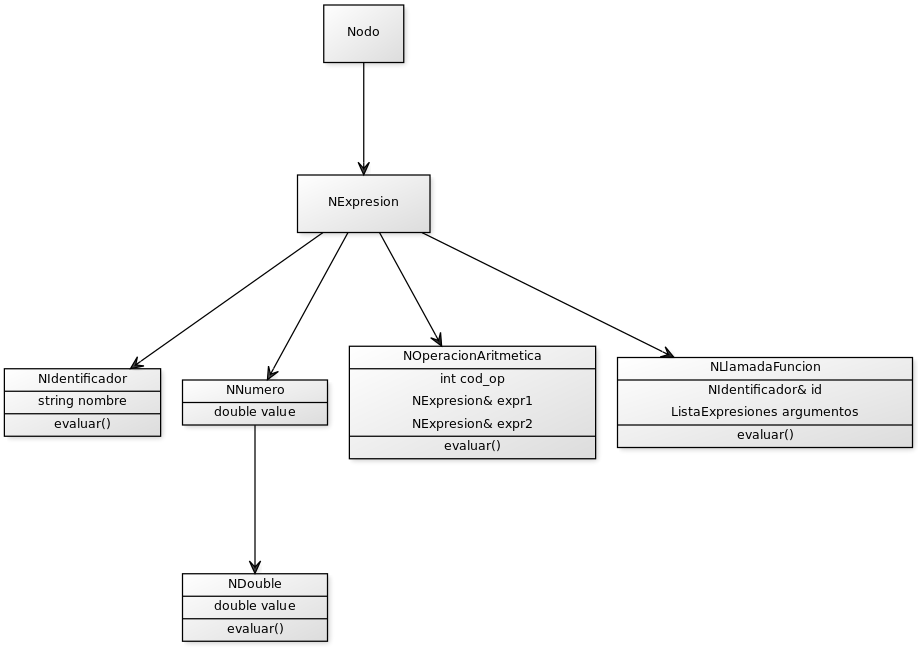
\includegraphics[width=0.9\textwidth,height=0.9\textheight,keepaspectratio]{imgs/clases3.png}

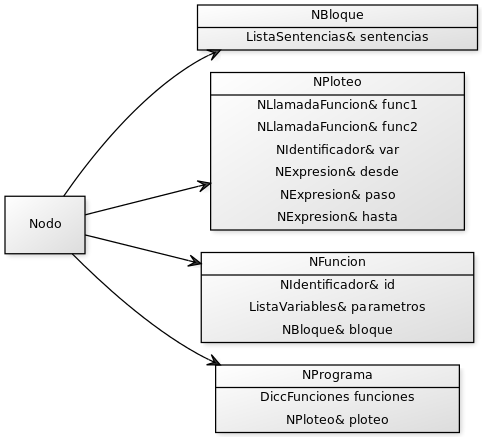
\includegraphics[width=0.9\textwidth,height=0.9\textheight,keepaspectratio]{imgs/clases4.png}
\newpage
\subsection{Diagrama de secuencia}
Este diagrama muestra una ejecución típica de nuestro intérprete/graficador.\\
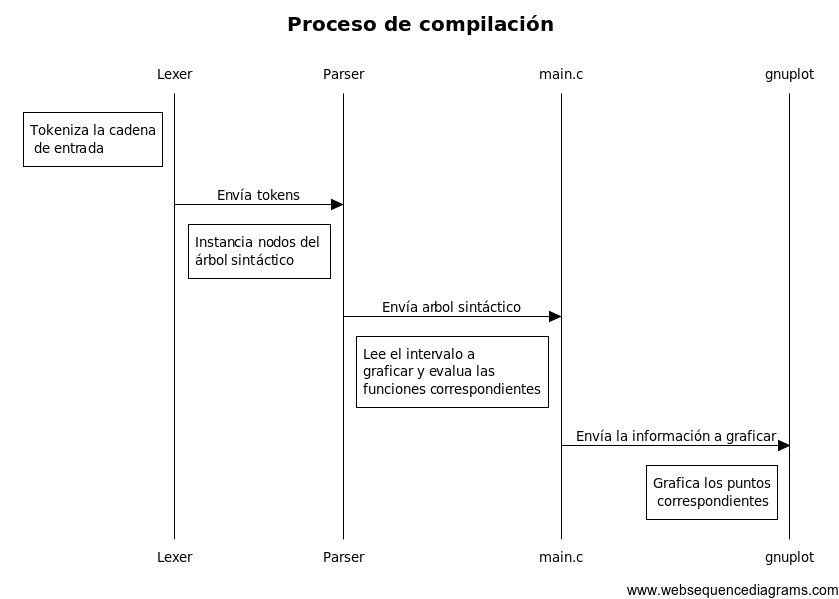
\includegraphics[width=0.9\textwidth,height=0.9\textheight,keepaspectratio]{imgs/secuencia.png}

Modo de uso:
\begin{verbatim}
make clean && make
cat archivodetest.cod | ./parser | ./graficador.sh 
\end{verbatim} 